\documentclass[11pt,a4paper]{article}

\usepackage[margin=2.1cm]{geometry}
\usepackage[T1]{fontenc}
\usepackage{lmodern}
\usepackage{amsmath,amssymb,bm}
\usepackage{booktabs}
\usepackage{array}
\usepackage{xcolor}
\usepackage{tikz}
\usetikzlibrary{arrows.meta,positioning,fit,calc,backgrounds}
\usepackage{caption}
\usepackage{enumitem}
\usepackage{listings}
\usepackage[most]{tcolorbox}
\usepackage{algorithm}
\usepackage{algpseudocode}
\usepackage[section]{placeins}
\usepackage{hyperref}
\hypersetup{colorlinks=true,linkcolor=blue!50!black,urlcolor=blue!50!black,citecolor=blue!50!black}

\definecolor{aa}{HTML}{1F77B4}
\definecolor{glob}{HTML}{D62728}
\definecolor{ok}{HTML}{2CA02C}
\definecolor{tr}{HTML}{9467BD}

\lstset{language=Python, basicstyle=\ttfamily\scriptsize, keywordstyle=\color{aa!80!black}\bfseries,
  commentstyle=\color{gray}\itshape, stringstyle=\color{ok!60!black}, columns=fullflexible, keepspaces=true,
  frame=l, framerule=1.2pt, rulecolor=\color{aa!50}, xleftmargin=8pt, numbers=left, numberstyle=\tiny\color{gray},
  showstringspaces=false, aboveskip=4pt, belowskip=4pt}

% file reference
\newcommand{\src}[1]{\texttt{\small #1}}
\sloppy
\setlength{\emergencystretch}{3em}

% Phase card: Code / Input / Output / How
\newenvironment{card}[1]{%
  \begin{tcolorbox}[enhanced,colback=aa!3,colframe=aa!65!black,fonttitle=\bfseries\small,title={#1},
    left=4pt,right=4pt,top=3pt,bottom=3pt,boxrule=0.6pt,arc=2pt]\small
  \begin{tabular}{@{}>{\bfseries}p{1.7cm}p{\dimexpr\linewidth-1.7cm-2\tabcolsep\relax}@{}}}%
  {\end{tabular}\end{tcolorbox}}

% Pipeline strip with one phase highlighted (1-7 inference, 8-12 training/evaluation)
\newcommand{\strip}[1]{%
\begin{center}
\begin{tikzpicture}[font=\tiny, every node/.style={align=center}]
\foreach \i/\t [count=\k] in {1/{Input \&\\patchify},2/{Token\\assembly},3/{Alternating\\Attention},4/{Camera\\head},
  5/{Pose\\decoding},6/{DPT dense\\heads},7/{Depth+cam\\$\to$ points}} {
  \ifnum\i=#1 \def\fillc{aa!45}\def\drawc{aa!80!black}\else\def\fillc{gray!8}\def\drawc{gray!50}\fi
  \node[draw=\drawc, fill=\fillc, rounded corners=1.5pt, minimum width=16mm, minimum height=7mm, thick]
    (s\i) at (\k*1.95,0) {\textbf{\i}\;\t};
  \ifnum\i>1 \pgfmathtruncatemacro{\j}{\i-1}\draw[-{Stealth[length=1.2mm]}, gray] (s\j) -- (s\i);\fi
}
\foreach \i/\t [count=\k] in {8/{Synthetic\\data},9/{Loss},10/{Training\\loop},11/{Evaluation\\metrics},12/{SIFT\\baseline}} {
  \ifnum\i=#1 \def\fillc{tr!40}\def\drawc{tr!80!black}\else\def\fillc{gray!8}\def\drawc{gray!50}\fi
  \node[draw=\drawc, fill=\fillc, rounded corners=1.5pt, minimum width=16mm, minimum height=7mm, thick]
    (s\i) at (\k*1.95+1.95,-1.0) {\textbf{\i}\;\t};
}
\end{tikzpicture}
\end{center}}

\title{\textbf{VGGT Code Walkthrough}\\[4pt]
\large From images to cameras, depth and point maps: inputs, outputs, implementation\\
and mathematics of every phase of the pipeline}
\author{Platinum-Saber/VGGT, code review notes}
\date{November 2026}

\begin{document}
\maketitle

\begin{abstract}
This document accompanies a code review of the repository's from-scratch re-implementation of VGGT
(Visual Geometry Grounded Transformer, Wang et al., CVPR 2025). The architecture diagram is split into seven inference
phases and five training/evaluation phases. For each phase we give the source location, the tensors that enter and leave it
(with shapes for the released VGGT-1B configuration and for the 10.7\,M-parameter model trained in this project), how the code
achieves the transformation, and the underlying mathematics or algorithm. Line numbers refer to the code on
branch \texttt{claude/clever-curie-rl6bco}.
\end{abstract}

\tableofcontents
\newpage

%==========================================================================================
\section{Overview and notation}

\subsection{The pipeline at a glance}

VGGT is a single feed-forward network
\[
  f\big((I_i)_{i=1}^{S}\big) = \big(\mathbf{g}_i,\; D_i,\, \Sigma^D_i,\; P_i,\, \Sigma^P_i\big)_{i=1}^{S},
\]
mapping $S$ RGB images of one scene to, per frame, a camera $\mathbf{g}_i$ (extrinsics and intrinsics), a depth map $D_i$,
a point map $P_i$ expressed in the coordinate frame of the \emph{first} camera, and confidence maps for both. (The paper's
tracking head is not part of this repository.) Figure~\ref{fig:arch} shows the architecture with the phase numbers used
in the rest of this document; Table~\ref{tab:files} maps every phase to its source file.

\begin{figure}[htbp]
\centering
\resizebox{\linewidth}{!}{%
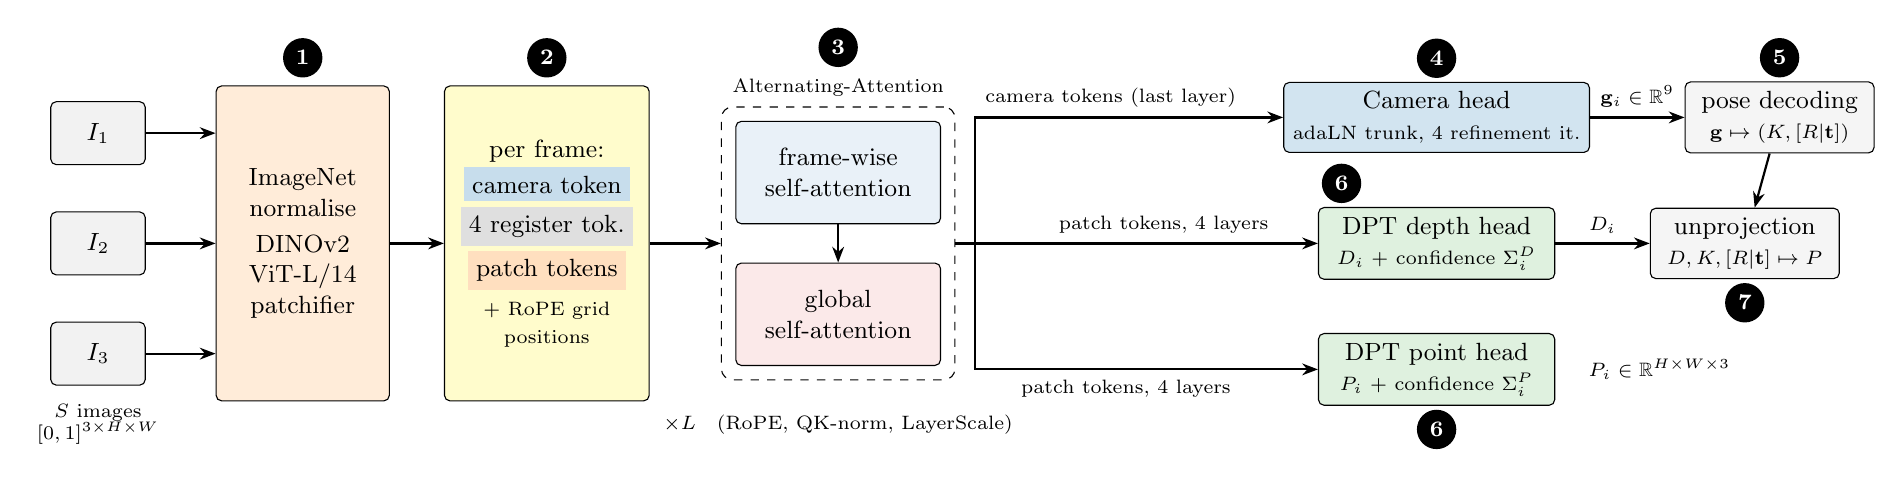
\begin{tikzpicture}[
  font=\small,
  box/.style={draw, rounded corners=2pt, minimum height=8mm, align=center, fill=#1},
  box/.default=white,
  arr/.style={-{Stealth[length=2mm]}, thick},
  lab/.style={font=\scriptsize, align=center},
  num/.style={circle, fill=black, text=white, inner sep=1pt, minimum size=5mm, font=\footnotesize\bfseries}
]
\foreach \i/\y in {1/1.4,2/0.0,3/-1.4} { \node[box=gray!10, minimum width=12mm] (img\i) at (0,\y) {$I_{\i}$}; }
\node[lab] at (0,-2.3) {$S$ images\\$[0,1]^{3\times H\times W}$};
\node[box=orange!15, minimum width=22mm, minimum height=40mm] (dino) at (2.6,0) {ImageNet\\normalise\\[2pt]DINOv2\\ViT-L/14\\patchifier};
\foreach \i in {1,2,3} { \draw[arr] (img\i) -- (dino.west |- img\i); }
\node[box=yellow!20, minimum width=26mm, minimum height=40mm] (tok) at (5.7,0) {per frame:\\[2pt]
  \colorbox{aa!25}{camera token}\\[1pt]\colorbox{gray!25}{4 register tok.}\\[1pt]\colorbox{orange!25}{patch tokens}\\[3pt]
  \scriptsize + RoPE grid\\[-1pt]\scriptsize positions};
\draw[arr] (dino) -- (tok);
\node[box=aa!10, minimum width=26mm, minimum height=13mm] (fa) at (9.4,0.9) {frame-wise\\self-attention};
\node[box=glob!10, minimum width=26mm, minimum height=13mm] (ga) at (9.4,-0.9) {global\\self-attention};
\draw[arr] (fa) -- (ga);
\node[draw, dashed, rounded corners, fit=(fa)(ga), inner sep=5pt, label={[lab]above:Alternating-Attention}] (aa) {};
\node[lab] at (9.4,-2.3) {$\times L$ \; (RoPE, QK-norm, LayerScale)};
\draw[arr] (tok) -- (aa.west |- tok);
\node[box=aa!20, minimum width=30mm] (cam) at (17.0,1.6) {Camera head\\\scriptsize adaLN trunk, 4 refinement it.};
\node[box=ok!15, minimum width=30mm] (dep) at (17.0,0) {DPT depth head\\\scriptsize $D_i$ + confidence $\Sigma^D_i$};
\node[box=ok!15, minimum width=30mm] (pts) at (17.0,-1.6) {DPT point head\\\scriptsize $P_i$ + confidence $\Sigma^P_i$};
\coordinate (aaout) at ($(aa.east)+(0.25,0)$);
\draw[thick] (aa.east) -- (aaout);
\draw[arr] (aaout) |- node[lab, pos=0.72, above] {camera tokens (last layer)} (cam.west);
\draw[arr] (aaout) -- node[lab, above, pos=0.55] {patch tokens, 4 layers} (dep.west);
\draw[arr] (aaout) |- node[lab, pos=0.72, below] {patch tokens, 4 layers} (pts.west);
\node[box=gray!8, minimum width=24mm, right=12mm of cam] (dec) {pose decoding\\\scriptsize $\mathbf{g}\mapsto(K,[R|\mathbf{t}])$};
\draw[arr] (cam) -- node[lab, above] {$\mathbf{g}_i\in\mathbb{R}^9$} (dec);
\node[box=gray!8, minimum width=24mm, right=12mm of dep] (unp) {unprojection\\\scriptsize $D, K, [R|\mathbf{t}]\mapsto P$};
\draw[arr] (dep) -- node[lab, above] {$D_i$} (unp);
\draw[arr] (dec) -- (unp);
\node[lab, right=3mm of pts] {$P_i\in\mathbb{R}^{H\times W\times 3}$};
% phase numbers
\node[num] at ($(dino.north)+(0,0.35)$) {1};
\node[num] at ($(tok.north)+(0,0.35)$) {2};
\node[num] at ($(aa.north)+(0,0.75)$) {3};
\node[num] at ($(cam.north)+(0,0.3)$) {4};
\node[num] at ($(dec.north)+(0,0.3)$) {5};
\node[num] at ($(pts.south)+(0,-0.3)$) {6};
\node[num] at ($(dep.north west)+(0.3,0.3)$) {6};
\node[num] at ($(unp.south)+(0,-0.3)$) {7};
\end{tikzpicture}}
\caption{Architecture as implemented, segmented into the inference phases 1--7 (black circles) discussed in
Sections~\ref{sec:p1}--\ref{sec:p7}. Phases 8--12 (data, loss, training loop, evaluation, classical baseline) wrap around this
network and are covered in Sections~\ref{sec:p8}--\ref{sec:p12}.}
\label{fig:arch}
\end{figure}

\begin{table}[htbp]
\centering
\caption{Phase-to-code map.}
\label{tab:files}
\footnotesize
\begin{tabular}{c>{\raggedright}p{3.4cm}>{\raggedright}p{6.2cm}>{\raggedright\arraybackslash}p{4.4cm}}
\toprule
& Phase & Main code & Entry point \\
\midrule
1 & Input normalisation, patchify & \src{vggt/aggregator.py:85--87}, \src{vggt/dino.py}, \src{vggt/layers.py:131} & \texttt{Aggregator.forward} \\
2 & Token assembly, positions & \src{vggt/aggregator.py:90--100, 123--127}, \src{layers.py:38} & \texttt{Aggregator.forward} \\
3 & Alternating-Attention & \src{vggt/aggregator.py:102--120}, \src{vggt/layers.py:53--128} & \texttt{Aggregator.forward} \\
4 & Camera head & \src{vggt/heads/camera\_head.py} & \texttt{CameraHead.forward} \\
5 & Pose decoding & \src{vggt/utils/pose\_enc.py}, \src{vggt/utils/rotation.py} & \texttt{pose\_encoding\_to\_\allowbreak extri\_intri} \\
6 & DPT dense heads & \src{vggt/heads/dpt\_head.py} & \texttt{DPTHead.forward} \\
7 & Depth + camera $\to$ points & \src{vggt/utils/geometry.py} & \texttt{unproject\_depth\_to\_world} \\
\midrule
8 & Synthetic data & \src{training/synthetic.py} & \texttt{SceneSampler}, \texttt{MultiViewDataset} \\
9 & Loss & \src{training/losses.py} & \texttt{vggt\_loss} \\
10 & Training loop & \src{training/train.py} & \texttt{main} \\
11 & Evaluation metrics & \src{training/metrics.py}, \src{training/evaluate.py} & \texttt{evaluate} \\
12 & SIFT baseline & \src{training/baseline\_sift.py} & \texttt{rel\_pose} \\
\bottomrule
\end{tabular}
\end{table}

\subsection{Top-level forward pass}

\src{vggt/model.py:69--83} wires the phases together. The aggregator returns a list of per-layer token tensors; each head reads
what it needs from that list.

\begin{lstlisting}[firstnumber=69]
def forward(self, images, num_camera_iterations=4):
    if images.dim() == 4:
        images = images[None]                       # (S,3,H,W) -> (1,S,3,H,W)
    tokens, patch_start_idx = self.aggregator(images)                       # phases 1-3
    preds = {}
    if self.camera_head is not None:                                         # phase 4
        pose_enc_list = self.camera_head(tokens, num_iterations=num_camera_iterations)
        preds["pose_enc"] = pose_enc_list[-1]
        preds["pose_enc_list"] = pose_enc_list
    if self.depth_head is not None:                                          # phase 6
        preds["depth"], preds["depth_conf"] = self.depth_head(tokens, images, patch_start_idx)
    if self.point_head is not None:
        preds["world_points"], preds["world_points_conf"] = self.point_head(tokens, images, patch_start_idx)
    return preds
\end{lstlisting}

\subsection{Notation and the two configurations}

$B$ batch size, $S$ frames per scene, $H\times W$ image size, $p=14$ patch size, $h=H/p$, $w=W/p$, $K=hw$ patches per frame,
$P = 1 + 4 + K$ tokens per frame (camera, 4 registers, patches), $C$ token width, $L$ aggregator depth.
\texttt{VGGT()} with default arguments is the released VGGT-1B; \texttt{VGGT.small()} (\src{model.py:56--67}) is the
model trained in this project.

\begin{table}[htbp]
\centering
\caption{Configurations and the resulting token shapes (square inputs).}
\label{tab:configs}
\small
\begin{tabular}{lcc}
\toprule
 & VGGT-1B (\texttt{VGGT()}) & small (\texttt{VGGT.small()}) \\
\midrule
Input $H\times W$ & $518\times518$ & $112\times112$ \\
Patchifier & DINOv2 ViT-L/14 + 4 registers & single $14\times14$ conv \\
Patch grid $h\times w$, $K$ & $37\times37$, 1369 & $8\times8$, 64 \\
Tokens per frame $P$ & 1374 & 69 \\
Width $C$ / heads / head dim & 1024 / 16 / 64 & 192 / 6 / 32 \\
AA depth $L$ & 24 (frame + global) & 6 + 6 (AA) or 12 global (ablation) \\
Layers read by DPT & $\{4, 11, 17, 23\}$ & $\{1, 2, 3, 5\}$ \\
DPT channels (features) & $(256, 512, 1024, 1024)$ (256) & $(32, 64, 128, 128)$ (32) \\
Camera trunk & 4 blocks, 16 heads & 2 blocks, 6 heads \\
Parameters & $\approx$1.18\,B (no tracking head) & 10.66\,M \\
\bottomrule
\end{tabular}
\end{table}

Table~\ref{tab:trace} traces the tensor shapes through one forward pass; the following sections explain each step.

\begin{table}[htbp]
\centering
\caption{Tensor shapes through one forward pass for VGGT-1B with $B=1$, $S=4$, $518\times518$ inputs (small model in brackets,
$112\times112$).}
\label{tab:trace}
\small
\begin{tabular}{clll}
\toprule
Phase & Tensor & VGGT-1B & [small] \\
\midrule
1 & input images & $(1,4,3,518,518)$ & $[(1,4,3,112,112)]$ \\
1 & patch tokens & $(4,1369,1024)$ & $[(4,64,192)]$ \\
2 & tokens + specials & $(4,1374,1024)$ & $[(4,69,192)]$ \\
3 & frame-attention sequence & $(4,1374,1024)$ & $[(4,69,192)]$ \\
3 & global-attention sequence & $(1,5496,1024)$ & $[(1,276,192)]$ \\
3 & stored layer output & $(1,4,1374,2048)$ & $[(1,4,69,384)]$ \\
4 & camera tokens & $(1,4,2048)$ & $[(1,4,384)]$ \\
4 & pose encodings & $4\times(1,4,9)$ & $[4\times(1,4,9)]$ \\
5 & extrinsics / intrinsics & $(1,4,3,4)$ / $(1,4,3,3)$ & same \\
6 & DPT pyramid & $148^2, 74^2, 37^2, 19^2$ & $[32^2, 16^2, 8^2, 4^2]$ \\
6 & depth, depth conf. & $(1,4,518,518,1)$, $(1,4,518,518)$ & $[(1,4,112,112,1)]$ \\
6 & points, points conf. & $(1,4,518,518,3)$, $(1,4,518,518)$ & $[(1,4,112,112,3)]$ \\
7 & unprojected points & $(4,518,518,3)$ & $[(4,112,112,3)]$ \\
\bottomrule
\end{tabular}
\end{table}

%==========================================================================================
\section{Phase 1: Input normalisation and patchification}\label{sec:p1}
\strip{1}

\begin{card}{Phase 1 at a glance}
Code & \src{aggregator.py:85--87}; \src{dino.py:25--75} (VGGT-1B); \src{layers.py:131--141} (small) \\
Input & images $\in[0,1]^{B\times S\times 3\times H\times W}$, $H, W$ multiples of 14 \\
Output & patch tokens $\in\mathbb{R}^{(B S)\times K\times C}$ \\
How & per-channel ImageNet normalisation, frames folded into the batch axis, then a ViT patchifier \\
\end{card}

\paragraph{Normalisation.} Every pixel is standardised with the ImageNet statistics used to pre-train DINOv2,
$\tilde{x}_c = (x_c - \mu_c)/\sigma_c$, $\bm\mu = (0.485, 0.456, 0.406)$, $\bm\sigma = (0.229, 0.224, 0.225)$, stored as
non-persistent buffers so they are not part of the checkpoint (\src{aggregator.py:75--76}). The $S$ frames are then reshaped into
the batch axis, $(B,S,3,H,W)\to(BS,3,H,W)$: the patchifier sees each frame independently.

\paragraph{Patch embedding.} A convolution with kernel size $=$ stride $=p$ is exactly a shared linear map applied to
each non-overlapping $p\times p$ patch:
\[
  \mathbf{e}_k = W_{\text{pe}}\,\operatorname{vec}\!\big(\tilde{I}[\text{patch }k]\big) + \mathbf{b},\qquad
  W_{\text{pe}}\in\mathbb{R}^{C\times 3p^2},\; k=1,\dots,K .
\]
\texttt{PatchEmbed} implements this as \texttt{Conv2d(3, C, p, stride=p)} followed by \texttt{flatten(2).transpose(1,2)}.
The small model stops here.

\paragraph{DINOv2 (VGGT-1B).} \texttt{DinoVisionTransformer.forward} (\src{dino.py:66--75}) reproduces DINOv2-with-registers:
\begin{enumerate}[nosep]
  \item patch-embed as above, prepend a learned \texttt{cls} token;
  \item add learned absolute position embeddings. They were trained on a $37\times37$ grid; for other grids the patch part is
        resampled with bicubic, anti-aliased interpolation (\texttt{interpolate\_pos\_encoding}, \src{dino.py:51--64});
  \item insert 4 register tokens after \texttt{cls} (registers absorb the high-norm ``artefact'' activations of plain ViTs);
  \item 24 pre-norm transformer blocks (Phase~3 block, without RoPE/QK-norm), final LayerNorm;
  \item return only the $K$ normalised patch tokens, \texttt{x[:, 1 + num\_register\_tokens:]}.
\end{enumerate}
The \texttt{cls} and DINO register outputs are discarded; VGGT adds its own special tokens in Phase~2.

%==========================================================================================
\section{Phase 2: Token assembly and positions}\label{sec:p2}
\strip{2}

\begin{card}{Phase 2 at a glance}
Code & \src{aggregator.py:70--73} (parameters), \src{aggregator.py:90--100}, \texttt{\_first\_vs\_rest} (\src{123--127}),
\texttt{PositionGetter} (\src{layers.py:38--50}) \\
Input & patch tokens $(BS, K, C)$ \\
Output & tokens $(BS, P, C)$ with $P=1+4+K$; integer positions $(BS, P, 2)$; \texttt{patch\_start\_idx} $=5$ \\
How & prepend 1 camera and 4 register tokens per frame, chosen from two learned sets (reference frame vs.\ others) \\
\end{card}

\paragraph{Reference-frame tokens.} The camera token has shape $(1,2,1,C)$ and the register tokens $(1,2,4,C)$. Slot 0 is used
for frame 1, slot 1 for every other frame:

\begin{lstlisting}[firstnumber=123]
def _first_vs_rest(token, B, S):
    """(1, 2, X, C) -> (B*S, X, C): slot 0 for frame 0, slot 1 for frames 1..S-1."""
    first = token[:, :1].expand(B, 1, *token.shape[2:])
    rest = token[:, 1:].expand(B, S - 1, *token.shape[2:])
    return torch.cat([first, rest], dim=1).reshape(B * S, *token.shape[2:])
\end{lstlisting}

This is the only place where frame order matters. Because the outputs are expressed in the first camera's coordinate system, the
network must know which frame is the reference; all other frames are treated symmetrically, so the model is
permutation-equivariant in frames $2,\dots,S$. The tokens are initialised with $\mathcal{N}(0,10^{-12})$ noise.

\paragraph{Positions for RoPE.} \texttt{PositionGetter} returns the $(y,x)$ grid index of every patch (cached per grid size).
The aggregator shifts them by $+1$ and gives the five special tokens position $(0,0)$:
\[
  \text{pos}(\text{patch at row } r, \text{column } c) = (r+1,\, c+1), \qquad \text{pos}(\text{special}) = (0,0).
\]
Position 0 means a rotation by angle 0, i.e.\ special tokens are not rotated (Phase~3). Positions are per-frame grid
coordinates, so the same pixel location in two different frames has the same position.

%==========================================================================================
\section{Phase 3: Alternating-Attention aggregator}\label{sec:p3}
\strip{3}

\begin{card}{Phase 3 at a glance}
Code & \src{aggregator.py:102--120} (loop), \src{layers.py:113--128} (\texttt{Block}), \src{90--110} (\texttt{Attention}),
\src{53--87} (\texttt{RotaryPositionEmbedding2D}) \\
Input & tokens $(BS, P, C)$, positions $(BS, P, 2)$ \\
Output & list of $L$ entries; entry $i$ is $(B, S, P, 2C)$ $=[\text{frame output}\,\|\,\text{global output}]$ for layers
read by a head, otherwise \texttt{None}; plus \texttt{patch\_start\_idx} \\
How & $L$ pairs of transformer blocks; the frame block attends within each image, the global block across all images,
implemented purely by reshaping the token tensor \\
\end{card}

\subsection{The alternating loop}

\begin{lstlisting}[firstnumber=103]
for i in range(self.depth):
    inter = []
    for attn_type in self.aa_order:
        if attn_type == "frame":   # attention within each frame: (B*S, P, C)
            tokens = self._run(self.frame_blocks[i], tokens.reshape(B * S, P, C),
                               None if pos is None else pos.reshape(B * S, P, 2))
        elif attn_type == "global":  # attention across all frames: (B, S*P, C)
            tokens = self._run(self.global_blocks[i], tokens.reshape(B, S * P, C),
                               None if pos is None else pos.reshape(B, S * P, 2))
        inter.append(tokens.reshape(B, S, P, C))
    if self.cached_layer_indices is None or i in self.cached_layer_indices:
        outputs.append(torch.cat(inter if len(inter) == 2 else inter * 2, dim=-1))
    else:
        outputs.append(None)
\end{lstlisting}

The two attention types are the same \texttt{Block}; they differ only in the sequence the attention sees:
\begin{itemize}[nosep]
  \item \textbf{frame-wise}: $(BS, P, C)$, each sequence is one image. Cost $\propto B\,S\,P^2 C$.
  \item \textbf{global}: $(B, SP, C)$, one sequence holds all tokens of all frames. Cost $\propto B\,(SP)^2 C$, which is
        what makes inference time grow super-linearly with $S$ (for VGGT-1B with $S=8$ the global sequence has 10\,992 tokens).
\end{itemize}
Only layers that some head reads are kept (\texttt{cached\_layer\_indices} plus the last layer), saving memory.
For the global-only ablation (\texttt{aa\_order=("global",)}) there is one output per layer, duplicated so the heads still
receive $2C$ channels; the model then has $2L$ global blocks if built with \texttt{depth=2L}, matching the AA parameter count.
During training each block can be wrapped in activation checkpointing (\texttt{\_run}, \src{aggregator.py:78--81}).

\begin{algorithm}[htbp]
\caption{Alternating-Attention aggregator}
\begin{algorithmic}[1]
\Require tokens $X\in\mathbb{R}^{B\times S\times P\times C}$, positions $\Pi$
\For{$i = 0,\dots,L-1$}
  \State $X \gets \mathrm{Block}^{\text{frame}}_i\big(X.\mathrm{reshape}(BS, P, C),\ \Pi\big)$ \Comment{intra-image}
  \State $F_i \gets X.\mathrm{reshape}(B,S,P,C)$
  \State $X \gets \mathrm{Block}^{\text{global}}_i\big(X.\mathrm{reshape}(B, SP, C),\ \Pi\big)$ \Comment{inter-image}
  \State $G_i \gets X.\mathrm{reshape}(B,S,P,C)$
  \State \textbf{if} $i$ is read by a head \textbf{then} store $Z_i = [F_i \,\|\, G_i] \in \mathbb{R}^{B\times S\times P\times 2C}$
\EndFor
\State \Return $(Z_i)_i$, \texttt{patch\_start\_idx}$=5$
\end{algorithmic}
\end{algorithm}

\subsection{Transformer block}

Each block is a pre-norm ViT block with LayerScale (\src{layers.py:126--128}):
\[
  X \leftarrow X + \bm\gamma_1 \odot \operatorname{Attn}\!\big(\operatorname{LN}_1(X)\big),\qquad
  X \leftarrow X + \bm\gamma_2 \odot \operatorname{MLP}\!\big(\operatorname{LN}_2(X)\big),
\]
with $\operatorname{MLP}(x) = W_2\,\operatorname{GELU}(W_1 x)$, hidden width $4C$, and LayerScale vectors
$\bm\gamma_{1,2}$ initialised to $0.01$ so each block starts close to the identity.

\paragraph{Multi-head attention with QK-norm and RoPE.} For $n_h$ heads of width $d=C/n_h$ (\src{layers.py:103--110}):
\begin{gather*}
  [Q,K,V] = X W_{qkv},\qquad \hat{Q} = \mathcal{R}_{\Pi}\big(\operatorname{LN}(Q)\big),\qquad
  \hat{K} = \mathcal{R}_{\Pi}\big(\operatorname{LN}(K)\big),\\
  \operatorname{Attn}(X) = W_o\,\operatorname{softmax}\!\Big(\frac{\hat{Q}\hat{K}^\top}{\sqrt{d}}\Big)V ,
\end{gather*}
computed per head with \texttt{F.scaled\_dot\_product\_attention}. The LayerNorm over the head dimension on $Q$ and $K$
(QK-norm) bounds the attention logits and stabilises training at large scale.

\paragraph{2D rotary position embedding.} $\mathcal{R}_\Pi$ rotates the first half of each head's channels by the row index
$y$ and the second half by the column index $x$ (\src{layers.py:80--87}). For one axis with $d' = d/2$ channels and integer
position $m$, the code uses the ``rotate-half'' form with frequencies $\theta_j = b^{-2j/d'}$, $b = 100$,
$j = 0,\dots,d'/2-1$, and $\bm\Theta = [\bm\theta, \bm\theta]$:
\[
  \mathcal{R}_m(\mathbf{x}) = \mathbf{x}\odot\cos(m\bm\Theta) + \operatorname{rot}(\mathbf{x})\odot\sin(m\bm\Theta),
  \qquad \operatorname{rot}([\mathbf{x}_1;\mathbf{x}_2]) = [-\mathbf{x}_2;\mathbf{x}_1].
\]
This rotates each channel pair $(x_j, x_{j+d'/2})$ by angle $m\theta_j$, i.e.\ $\mathcal{R}_m$ is block-diagonal
orthogonal with $\mathcal{R}_m^\top\mathcal{R}_n = \mathcal{R}_{n-m}$. Hence
\[
  \big\langle \mathcal{R}_m\mathbf{q},\, \mathcal{R}_n\mathbf{k}\big\rangle = \big\langle \mathbf{q},\, \mathcal{R}_{n-m}\mathbf{k}\big\rangle ,
\]
so the attention logit depends only on the \emph{relative} offset of two patches inside the image. Special tokens have
$m=0$ (identity). In global attention two tokens from different frames at the same pixel location have relative offset zero:
RoPE encodes where a patch is within its image, and the network must learn cross-view relations from content. The cosine/sine
tables are cached per (dimension, length, device, dtype).

%==========================================================================================
\section{Phase 4: Camera head}\label{sec:p4}
\strip{4}

\begin{card}{Phase 4 at a glance}
Code & \src{vggt/heads/camera\_head.py:16--44} \\
Input & last aggregator layer, camera token only: $Z_{L-1}[:,:,0] \in \mathbb{R}^{B\times S\times 2C}$ \\
Output & list of 4 pose encodings $\hat{\mathbf{g}}^{(1)},\dots,\hat{\mathbf{g}}^{(4)} \in \mathbb{R}^{B\times S\times 9}$
(the last is the prediction; all are supervised) \\
How & iterative residual refinement: the current estimate modulates the camera tokens through adaptive LayerNorm, a small
transformer trunk mixes information across frames, an MLP outputs an update \\
\end{card}

\begin{lstlisting}[firstnumber=32]
tokens = self.token_norm(aggregated_tokens_list[-1][:, :, 0])  # (B, S, 2C) camera tokens
B, S, _ = tokens.shape
pred, preds = None, []
for _ in range(num_iterations):
    inp = self.embed_pose(self.empty_pose_tokens.expand(B, S, -1) if pred is None else pred.detach())
    shift, scale, gate = self.poseLN_modulation(inp).chunk(3, dim=-1)
    x = gate * (self.adaln_norm(tokens) * (1 + scale) + shift) + tokens
    delta = self.pose_branch(self.trunk_norm(self.trunk(x)))
    pred = delta if pred is None else pred + delta
    preds.append(torch.cat([pred[..., :7], F.relu(pred[..., 7:])], -1))
\end{lstlisting}

\paragraph{Mathematics.} Let $\mathbf{z}_i = \operatorname{LN}(\mathbf{c}_i)$ be the normalised camera token of frame $i$ and
$\mathbf{g}^{(0)}$ a learned ``empty'' pose vector. For $k = 1,\dots,4$:
\begin{align*}
  \mathbf{e}_i &= W_e\,\operatorname{sg}\big(\mathbf{g}_i^{(k-1)}\big) + \mathbf{b}_e, &
  [\bm\beta_i, \bm\alpha_i, \bm\gamma_i] &= W_m\,\operatorname{SiLU}(\mathbf{e}_i) + \mathbf{b}_m, \\
  \mathbf{x}_i &= \bm\gamma_i \odot \big(\operatorname{LN}_0(\mathbf{z}_i)\odot(1+\bm\alpha_i) + \bm\beta_i\big) + \mathbf{z}_i, &
  (\mathbf{h}_i)_{i} &= \operatorname{Trunk}\big((\mathbf{x}_i)_{i=1}^S\big), \\
  \mathbf{g}_i^{(k)} &= \mathbf{g}_i^{(k-1)} + \operatorname{MLP}\big(\operatorname{LN}(\mathbf{h}_i)\big), &
  \hat{\mathbf{g}}_i^{(k)} &= \big[\mathbf{g}^{(k)}_{i,1:7},\ \operatorname{ReLU}(\mathbf{g}^{(k)}_{i,8:9})\big],
\end{align*}
where $\operatorname{sg}$ is stop-gradient (\texttt{detach}), $\operatorname{LN}_0$ is a LayerNorm without affine parameters
(adaLN, as in DiT), and $\mathbf{g}^{(1)}$ is the first update itself. The trunk (4 or 2 \texttt{Block}s, no RoPE) attends
over the $S$ camera tokens, so each frame's update is conditioned on all other frames. The same trunk weights are reused in
every iteration. Stopping the gradient through the conditioning means each iteration learns ``given this estimate, how should
it change'', while gradients still reach earlier updates through the additive path $\mathbf{g}^{(k)}=\mathbf{g}^{(k-1)}+\Delta$.
The ReLU keeps the field of view non-negative.

%==========================================================================================
\section{Phase 5: Pose encoding and decoding}\label{sec:p5}
\strip{5}

\begin{card}{Phase 5 at a glance}
Code & \src{vggt/utils/pose\_enc.py}, \src{vggt/utils/rotation.py} \\
Input & $\hat{\mathbf{g}} \in \mathbb{R}^{\dots\times 9}$ and the image size $(H,W)$ \\
Output & extrinsics $[R\,|\,\mathbf{t}] \in \mathbb{R}^{\dots\times3\times4}$ (OpenCV camera-from-world) and intrinsics
$K\in\mathbb{R}^{\dots\times3\times3}$; the inverse map builds training targets \\
How & closed-form conversions: translation copied, quaternion $\leftrightarrow$ rotation matrix, field of view
$\leftrightarrow$ focal length \\
\end{card}

\paragraph{Encoding.} $\mathbf{g} = [\mathbf{t}\in\mathbb{R}^3,\ \mathbf{q} = (q_x,q_y,q_z,q_w)\in\mathbb{R}^4,\
\text{fov}_h,\ \text{fov}_w]$, with
\[
  \text{fov}_h = 2\arctan\frac{H/2}{f_y},\qquad \text{fov}_w = 2\arctan\frac{W/2}{f_x}.
\]
A point $\mathbf{X}$ in world (= first camera) coordinates maps to camera $i$ as $\mathbf{X}_{c} = R_i\mathbf{X} + \mathbf{t}_i$
and projects to $\mathbf{u} \sim K_i\mathbf{X}_c$. The first camera is therefore predicted as (approximately) the identity
pose; \texttt{results/kaggle/kitchen\_cameras.json} shows exactly that for the released model.

\paragraph{Decoding.} $f_x = \tfrac{W}{2}\big/\tan\tfrac{\text{fov}_w}{2}$, $f_y = \tfrac{H}{2}\big/\tan\tfrac{\text{fov}_h}{2}$,
principal point $(W/2, H/2)$, no skew. The rotation (\texttt{quat\_to\_mat}) is the standard formula for a not necessarily
unit quaternion $(i,j,k,r)$ with $s = 2/\|\mathbf{q}\|^2$:
\[
  R = \begin{pmatrix}
    1 - s(j^2+k^2) & s(ij - kr) & s(ik + jr)\\
    s(ij + kr) & 1 - s(i^2+k^2) & s(jk - ir)\\
    s(ik - jr) & s(jk + ir) & 1 - s(i^2+j^2)
  \end{pmatrix},
\]
which equals the rotation of $\mathbf{q}/\|\mathbf{q}\|$, so the network output need not be normalised.

\paragraph{Matrix to quaternion} (\texttt{mat\_to\_quat}, used to build targets) follows Shepperd's method: compute the four
candidates $|q_r|, |q_i|, |q_j|, |q_k|$ from $\sqrt{1\pm m_{00}\pm m_{11}\pm m_{22}}$, form the quaternion from the
largest one (best conditioned, avoids dividing by a value near 0), and finally flip the sign so that $q_w\ge0$. The
canonical sign matters for the loss, because $\mathbf{q}$ and $-\mathbf{q}$ are the same rotation but far apart in $L_1$.

%==========================================================================================
\section{Phase 6: DPT dense heads}\label{sec:p6}
\strip{6}

\begin{card}{Phase 6 at a glance}
Code & \src{vggt/heads/dpt\_head.py} (\texttt{DPTHead}, \texttt{FeatureFusionBlock}, \texttt{ResidualConvUnit},
\texttt{activate\_head}) \\
Input & patch tokens of 4 aggregator layers, $Z_\ell[:,:,5:] \in \mathbb{R}^{B\times S\times K\times 2C}$; images (for the size) \\
Output & depth head: $D \in \mathbb{R}_{>0}^{B\times S\times H\times W\times 1}$, $\Sigma^D \in [1,\infty)^{B\times S\times H\times W}$;
point head: $P \in \mathbb{R}^{B\times S\times H\times W\times 3}$, $\Sigma^P$ \\
How & DPT (Ranftl et al.): reassemble tokens into a 4-level feature pyramid, fuse coarse-to-fine with RefineNet blocks,
upsample to full resolution, apply output activations \\
\end{card}

Both dense heads are the same class; only the number of output channels and the activation differ
(\src{model.py:53--54}): the point head outputs $3+1$ channels with the inverse-log activation, the depth head $1+1$ channels
with $\exp$. Frames are processed in chunks of 8 to bound memory.

\begin{algorithm}[htbp]
\caption{DPT head (\texttt{DPTHead.\_forward}, \src{dpt\_head.py:140--166})}
\begin{algorithmic}[1]
\For{$n = 1..4$ with layer $\ell_n$}
  \State $F \gets \operatorname{LN}(Z_{\ell_n}[\text{patch tokens}])$, reshape to $(BS, 2C, h, w)$
  \State $F \gets \operatorname{Conv}_{1\times1}(F)$ to $c_n$ channels; $F \gets F + 0.1\cdot\operatorname{PE}_{uv}$
  \State resize: $n{=}1$: ConvT $4{\times}$ ($4h$); $n{=}2$: ConvT $2{\times}$ ($2h$); $n{=}3$: identity ($h$); $n{=}4$: Conv stride 2 ($h/2$)
  \State $L_n \gets \operatorname{Conv}_{3\times3}(F)$ to $c$ features
\EndFor
\State $O \gets \operatorname{Fuse}_4(L_4)$ upsampled to size of $L_3$
\State $O \gets \operatorname{Fuse}_3(O, L_3)$ to size of $L_2$;\quad $O \gets \operatorname{Fuse}_2(O, L_2)$ to size of $L_1$;\quad
       $O \gets \operatorname{Fuse}_1(O, L_1)$ (bilinear $2\times$)
\State $O \gets \operatorname{Conv}_{3\times3}(O)$ to $c/2$; bilinear resize to $H\times W$; $O \gets O + 0.1\cdot\operatorname{PE}_{uv}$
\State $O \gets \operatorname{Conv}_{1\times1}\big(\operatorname{ReLU}(\operatorname{Conv}_{3\times3}(O))\big)$ to $d_{\text{out}}+1$ channels
\State \Return $\operatorname{act}(O_{1:d_{\text{out}}})$, $\ 1 + \exp(O_{d_{\text{out}}+1})$
\end{algorithmic}
\end{algorithm}

\paragraph{Shapes.} For VGGT-1B ($h = 37$) the pyramid is $256@148^2$, $512@74^2$, $1024@37^2$, $1024@19^2$, fused at 256
channels to $296^2$, then resized to $518^2$. For the small model ($h=8$): $32@32^2$, $64@16^2$, $128@8^2$, $128@4^2$,
fused at 32 channels to $64^2$, resized to $112^2$.

\paragraph{Fusion block.} With $\operatorname{RCU}(x) = \operatorname{Conv}_2\big(\operatorname{ReLU}(\operatorname{Conv}_1(\operatorname{ReLU}(x)))\big) + \operatorname{ReLU}(x)$,
\[
  \operatorname{Fuse}(x, s) = \operatorname{Conv}_{1\times1}\Big(\operatorname{Up}\big(\operatorname{RCU}_2(x + \operatorname{RCU}_1(s))\big)\Big).
\]
The skip carrying $\operatorname{ReLU}(x)$ instead of $x$ is deliberate: the official code applies an in-place ReLU before the
residual, and the released weights depend on it (\src{dpt\_head.py:69--73}). Bit-exact agreement with the official
outputs (last section) requires reproducing such details.

\paragraph{UV positional embedding.} \texttt{create\_uv\_grid} gives each pixel coordinates
$(u,v)$ normalised by the image diagonal ($a=W/H$), and the embedding of a $c$-channel map is
\[
  (u,v)\in\Big[\tfrac{-a}{\sqrt{1+a^2}},\tfrac{a}{\sqrt{1+a^2}}\Big]\times\Big[\tfrac{-1}{\sqrt{1+a^2}},\tfrac{1}{\sqrt{1+a^2}}\Big],\qquad
  \operatorname{PE}_{uv} = 0.1\,\big[\sin(u\bm\omega), \cos(u\bm\omega), \sin(v\bm\omega), \cos(v\bm\omega)\big],
\]
with $\omega_k = 100^{-k/(c/4)}$, $k=0,\dots,c/4-1$. It re-injects absolute image position after the
token-to-image reshape.

\paragraph{Output activations.}
\[
  D = \exp(y), \qquad P = \operatorname{sign}(y)\,\big(e^{|y|} - 1\big), \qquad \Sigma = 1 + e^{c}.
\]
$\exp$ keeps depth positive and makes the network predict log-depth. The inverse-log map is the inverse of
$\operatorname{sign}(x)\log(1+|x|)$: it is near-linear around 0 (where the first camera's nearby points lie) and compresses
large coordinates. $\Sigma\ge1$ is the aleatoric confidence used by the loss (Phase~9) and to filter points at inference.

%==========================================================================================
\section{Phase 7: From depth and cameras to a point map}\label{sec:p7}
\strip{7}

\begin{card}{Phase 7 at a glance}
Code & \src{vggt/utils/geometry.py:25--35} (\texttt{unproject\_depth\_to\_world}), \texttt{inverse\_se3} (\src{6--14}) \\
Input & depth $D\in\mathbb{R}^{\dots\times H\times W}$, extrinsics $(\dots,3,4)$, intrinsics $(\dots,3,3)$ \\
Output & world points $\in\mathbb{R}^{\dots\times H\times W\times3}$ \\
How & back-project each pixel along its ray to the predicted depth, then map camera to world with the inverse rigid
transform \\
\end{card}

For pixel $(u,v)$ with depth $D_{uv}$:
\[
  \mathbf{X}_c = D_{uv}\,K^{-1}\begin{pmatrix}u\\v\\1\end{pmatrix}
  = \begin{pmatrix} (u - c_x)D_{uv}/f_x \\ (v - c_y)D_{uv}/f_y \\ D_{uv}\end{pmatrix},\qquad
  \mathbf{X}_w = R^\top(\mathbf{X}_c - \mathbf{t}),
\]
where the closed-form inverse $\begin{bmatrix}R & \mathbf{t}\end{bmatrix}^{-1} = \begin{bmatrix}R^\top & -R^\top\mathbf{t}\end{bmatrix}$
avoids a general matrix inverse. The same function is used in three places: to build the ground-truth point maps (Phase~8),
for the paper's ``depth + camera'' point maps in evaluation (Phase~11), and to export the coloured point cloud in
\src{scripts/demo\_pretrained.py} (keeping pixels above the 50th percentile of $\Sigma^D$). The paper (and our results) find
these points more accurate than the point head's direct output.

%==========================================================================================
\section{Phase 8: Synthetic multi-view data}\label{sec:p8}
\strip{8}

\begin{card}{Phase 8 at a glance}
Code & \src{training/synthetic.py}: \texttt{SceneSampler} (\src{42--168}), \texttt{normalize\_views} (\src{171--184}),
\texttt{generate\_dataset} (\src{187--199}), \texttt{MultiViewDataset} (\src{202--227}) \\
Input & random seed, number of scenes, image size (112), views per scene (6) \\
Output & per batch: images $(B,S,3,H,W)$, depths $(B,S,H,W)$, valid masks, world points $(B,S,H,W,3)$, extrinsics
$(B,S,3,4)$, intrinsics $(B,S,3,3)$, normalised to the first camera and unit mean point distance \\
How & a vectorised NumPy ray caster renders random rooms with spheres and boxes from cameras on an arc; ground truth is exact \\
\end{card}

\paragraph{Scenes and cameras.} A room is an axis-aligned box with half-extents in $[3,5]\times[2,3]\times[3,5]$, containing
3--6 spheres or boxes. Each view's camera sits at azimuth $\phi_0 \pm \tfrac12\text{spread}$ (spread $30^\circ$--$100^\circ$),
radius 1.9--2.6, height $-0.6$--$0.9$, and looks at a jittered target. \texttt{\_look\_at} builds the OpenCV frame
($x$ right, $y$ down, $z$ forward):
\[
  \mathbf{z} = \tfrac{\mathbf{o}-\mathbf{c}}{\|\mathbf{o}-\mathbf{c}\|},\quad
  \mathbf{x} = \tfrac{\mathbf{z}\times\mathbf{up}}{\|\mathbf{z}\times\mathbf{up}\|},\quad
  \mathbf{y} = \mathbf{z}\times\mathbf{x},\quad R = [\mathbf{x}\ \mathbf{y}\ \mathbf{z}]^\top,\quad \mathbf{t} = -R\mathbf{c},
\]
with $\mathbf{c}$ the camera centre and $\mathbf{o}$ the target. The field of view is drawn from $50^\circ$--$75^\circ$,
$f = \tfrac{W}{2}/\tan\tfrac{\text{fov}}{2}$.

\paragraph{Ray casting.} Each pixel's ray is $\mathbf{r}(\tau) = \mathbf{c} + \tau\mathbf{d}$ with
$\mathbf{d} = R^\top\big((u - W/2)/f,\ (v-H/2)/f,\ 1\big)^\top$. Because the camera-space direction has $z = 1$, the hit
parameter $\tau$ \emph{is} the depth. All pixels are intersected at once, keeping the nearest hit $\tau>10^{-4}$:
\begin{itemize}[nosep]
  \item \emph{walls} (seen from inside): $\tau = (\pm r_a - c_a)/d_a$ for each axis $a$;
  \item \emph{spheres}: solve $\|\mathbf{c} + \tau\mathbf{d} - \mathbf{m}\|^2 = \rho^2$, i.e.\ $a\tau^2 + b\tau + c' = 0$ with
        $a = \|\mathbf{d}\|^2$, $b = 2\mathbf{d}^\top(\mathbf{c}-\mathbf{m})$, $c' = \|\mathbf{c}-\mathbf{m}\|^2 - \rho^2$;
        nearest root $\tau = (-b - \sqrt{b^2 - 4ac'})/2a$ if the discriminant is positive;
  \item \emph{boxes}: slab method, $\tau_0 = (\mathbf{lo}-\mathbf{c})\oslash\mathbf{d}$, $\tau_1 = (\mathbf{hi}-\mathbf{c})\oslash\mathbf{d}$,
        $\tau_{\text{near}} = \max_a\min(\tau_0,\tau_1)_a$, $\tau_{\text{far}} = \min_a\max(\tau_0,\tau_1)_a$, hit iff
        $\tau_{\text{near}}\le\tau_{\text{far}}$; the normal is along the axis attaining $\tau_{\text{near}}$.
\end{itemize}
Colour is a \emph{solid} texture, a function of the 3D hit point (per-surface colour, sums of sinusoids, a 3D checkerboard),
times Lambertian shading $0.45 + 0.55\max(0, \mathbf{n}^\top\mathbf{l})$. Because appearance depends only on the 3D point,
it is consistent across views, so correspondences exist to be learned.

\paragraph{Storage and sampling.} Scenes are stored as \texttt{uint8} images and \texttt{fp16} depths (3000 training scenes:
1.36\,GB; 200 test scenes with a disjoint seed). \texttt{MultiViewDataset.batch} draws $B$ random scenes and $S$ random
views per scene; $S\in[2,6]$ is drawn once per step.

\paragraph{Normalisation} (as in the official training code). With homogeneous extrinsics $T_i$:
\begin{gather*}
  T_i \leftarrow T_i T_1^{-1}\ \ (\text{world} = \text{camera }1),\qquad
  \mathbf{X} = \operatorname{unproject}(D, T, K),\\
  s = \operatorname{mean}_{\text{valid}}\|\mathbf{X}\|,\qquad
  \mathbf{t}_i \leftarrow \mathbf{t}_i/s,\quad D\leftarrow D/s,\quad \mathbf{X}\leftarrow\mathbf{X}/s .
\end{gather*}
This removes the gauge freedom (global rigid motion and scale) that a multi-view network cannot observe.

%==========================================================================================
\section{Phase 9: Training objective}\label{sec:p9}
\strip{9}

\begin{card}{Phase 9 at a glance}
Code & \src{training/losses.py}: \texttt{camera\_loss} (\src{16--27}), \texttt{regression\_loss} (\src{52--65}),
\texttt{\_gradient\_loss} (\src{30--41}), \texttt{vggt\_loss} (\src{68--86}) \\
Input & model predictions (pose list, depth/points and confidences) and the batch from Phase~8 \\
Output & scalar objective and a dictionary of logged terms \\
How & $\mathcal{L} = 5\,\mathcal{L}_{\text{camera}} + \mathcal{L}_{\text{depth}} + \mathcal{L}_{\text{pmap}}$ \\
\end{card}

\paragraph{Camera loss.} Targets $\mathbf{g}$ are built with Phase~5's encoder. Over the $n = 4$ refinement outputs, with
$\gamma = 0.6$ (later iterations weigh more):
\[
  \mathcal{L}_{\text{camera}} = \frac{1}{n}\sum_{k=1}^{n}\gamma^{\,n-k}\Big(
  \overline{|\hat{\mathbf{t}}^{(k)} - \mathbf{t}|} + \overline{|\hat{\mathbf{q}}^{(k)} - \mathbf{q}|}
  + 0.5\,\overline{|\hat{\mathbf{f}}^{(k)} - \mathbf{f}|}\Big),
\]
where $\overline{\cdot}$ is the mean over elements and the translation error is clipped at 100. The paper states a Huber
loss; the official code (and this one) uses $L_1$.

\paragraph{Aleatoric-uncertainty regression.} For depth ($\mathbf{y}=D$) and points ($\mathbf{y}=P$), with per-pixel error
$e_j = \|\hat{\mathbf{y}}_j - \mathbf{y}_j\|_2$ over valid pixels and $\alpha = 0.2$:
\[
  \mathcal{L}_{\text{conf}} = \operatorname{mean}\big(\Sigma_j e_j - \alpha\log\Sigma_j\big),\qquad
  \mathcal{L}_{\text{reg}} = \operatorname{mean}(e_j),\qquad
  \mathcal{L}_{\text{grad}} = \frac14\sum_{s=0}^{3} \ell_{\nabla}\big(\text{every }2^s\text{-th pixel}\big),
\]
\[
  \ell_\nabla = \frac{1}{N_{\text{valid}}\,C}\sum_{j}\Big(\Sigma_j\,\big|\partial_x r_j\big| - \alpha\log\Sigma_j\Big)
  + (\text{same for }\partial_y),\qquad r = (\hat{\mathbf{y}} - \mathbf{y})\cdot\text{mask},
\]
and $\mathcal{L}_{\text{depth}} = \mathcal{L}_{\text{conf}}+\mathcal{L}_{\text{grad}}+\mathcal{L}_{\text{reg}}$ (same for points).
The gradient term rewards sharp, correctly placed discontinuities; the multi-scale version sees edges at several
resolutions. Before averaging, values above the 98th percentile are dropped (\texttt{\_quantile\_filter}) to ignore outliers
such as grazing-angle pixels.

\paragraph{Why the confidence term works.} For one pixel, minimising $\Sigma e - \alpha\log\Sigma$ over $\Sigma$ gives
$\partial_\Sigma = e - \alpha/\Sigma = 0 \Rightarrow \Sigma^\ast = \alpha/e$, i.e.\ the network learns to predict confidence
inversely proportional to its own error, and the optimal value $\alpha\big(1 + \log(e/\alpha)\big)$ grows only
logarithmically with $e$, making the loss robust. Since $\Sigma = 1 + e^{c}\ge 1$, pixels with $e > \alpha$ are pushed to
$\Sigma\to1$. Both $\mathcal{L}_{\text{conf}}$ and $\mathcal{L}_{\text{grad}}$ can be negative, which is why the logged
objective becomes negative late in training.

%==========================================================================================
\section{Phase 10: Training loop}\label{sec:p10}
\strip{10}

\begin{card}{Phase 10 at a glance}
Code & \src{training/train.py:35--106}; model factory \texttt{build\_model} (\src{30--32}) \\
Input & command-line config (model width/depth, \texttt{aa\_order}, steps, batch, lr, warm-up, device) \\
Output & \texttt{runs/<name>/config.json}, \texttt{log.jsonl} (every 50 steps), \texttt{model.pt} (every 1000 steps) \\
How & AdamW with decoupled weight decay, linear warm-up + cosine decay, gradient clipping, random frame count per step \\
\end{card}

\begin{algorithm}[htbp]
\caption{Training step (\src{train.py:87--106})}
\begin{algorithmic}[1]
\For{step $= 0,\dots,N-1$}
  \State set learning rate $\eta(\text{step})$ for all parameter groups
  \State $S \sim \mathcal{U}\{2,\dots,6\}$;\quad batch $\gets$ \texttt{ds.batch}$(B, S)$ \Comment{Phase 8}
  \State preds $\gets$ model(batch.images) \Comment{Phases 1--6}
  \State $\mathcal{L}\gets$ \texttt{vggt\_loss}(preds, batch) \Comment{Phase 9}
  \State backprop; clip $\|\nabla\|_2\le 1$; AdamW step
  \State every 50 steps: log; every 1000 steps: save checkpoint
\EndFor
\end{algorithmic}
\end{algorithm}

\paragraph{Learning-rate schedule.} With peak $\eta_0 = 4\times10^{-4}$, warm-up $N_w$ steps and progress
$\pi = (\text{step}-N_w)/(N - N_w)$:
\[
  \eta(\text{step}) = \begin{cases}
    \eta_0\,\dfrac{\text{step}+1}{N_w} & \text{step} < N_w,\\[6pt]
    \eta_0\Big(0.02 + 0.98\cdot\tfrac12\big(1+\cos\pi\pi\big)\Big) & \text{otherwise,}
  \end{cases}
\]
decaying to $2\%$ of the peak (the logged final value $8\times10^{-6}$). Weight decay $0.05$ is applied only to matrices
and kernels (\texttt{p.ndim >= 2}) that are not learned tokens; biases, norms, LayerScale and tokens are not decayed.
AdamW uses $\beta = (0.9, 0.95)$. CPU runs: batch 8, warm-up 300, 3k steps; Kaggle T4 runs: batch 16, warm-up 1000, 15k
steps (configs in \texttt{results/} and \texttt{results/kaggle/}).

%==========================================================================================
\section{Phase 11: Evaluation metrics}\label{sec:p11}
\strip{11}

\begin{card}{Phase 11 at a glance}
Code & \src{training/metrics.py}; driver \src{training/evaluate.py:20--50} \\
Input & checkpoint(s), held-out test scenes, frame counts $S\in\{2,4,6\}$ \\
Output & JSON with AUC@\{5,15,30\}, RRA@15, RTA@15, median errors, focal error, depth AbsRel and $\delta<1.25$,
point errors for the point head and for depth + camera \\
How & predicted poses are compared pairwise (gauge-invariant); depth after median scaling; points after a Sim(3) alignment \\
\end{card}

\paragraph{Relative pose errors.} For every ordered pair $i\ne j$, the relative transform $T_{ji} = T_j T_i^{-1}$
(camera $j$ from camera $i$) is computed for prediction and ground truth. Then
\[
  \varepsilon_R = \arccos\frac{\operatorname{tr}(\hat{R}_{ji}^\top R_{ji}) - 1}{2},\qquad
  \varepsilon_t = \arccos\frac{\hat{\mathbf{t}}_{ji}^\top\mathbf{t}_{ji}}{\|\hat{\mathbf{t}}_{ji}\|\,\|\mathbf{t}_{ji}\|}
\]
in degrees. Relative poses are independent of the world frame, and the translation \emph{direction} is independent of
scale, so no alignment is needed. RRA@15 / RTA@15 are the fractions of pairs below $15^\circ$.

\paragraph{AUC.} With $\varepsilon = \max(\varepsilon_R, \varepsilon_t)$ per pair and $M$ pairs,
\[
  \operatorname{AUC}@\tau = \frac{1}{\tau}\sum_{\theta=1}^{\tau}\frac{\#\{\varepsilon < \theta\}}{M},
\]
implemented with a 1-degree histogram and a cumulative sum (\src{metrics.py:40--45}).

\paragraph{Depth.} One median scale per sequence, $\hat D \leftarrow \hat D\cdot\operatorname{med}(D)/\operatorname{med}(\hat D)$,
then $\operatorname{AbsRel} = \operatorname{mean}|\hat D - D|/D$ and $\delta_{1.25} = \operatorname{mean}\big[\max(\hat D/D, D/\hat D) < 1.25\big]$.

\paragraph{Points: Umeyama alignment.} Predicted points are aligned to the ground truth with the least-squares similarity
$\min_{s,R,\mathbf{t}}\sum_j\|\mathbf{y}_j - (sR\mathbf{x}_j + \mathbf{t})\|^2$, solved in closed form
(\src{metrics.py:57--70}):
\[
  \Sigma_{xy} = \tfrac1N\sum_j(\mathbf{y}_j - \bm\mu_y)(\mathbf{x}_j - \bm\mu_x)^\top = U\,\mathrm{diag}(\mathbf{d})\,V^\top,\quad
  E = \mathrm{diag}\big(1,1,\operatorname{sign}\det(UV^\top)\big),
\]
\[
  R = UEV^\top,\qquad s = \frac{\operatorname{tr}(\mathrm{diag}(\mathbf{d})E)}{\tfrac1N\sum_j\|\mathbf{x}_j - \bm\mu_x\|^2},\qquad
  \mathbf{t} = \bm\mu_y - sR\bm\mu_x .
\]
$E$ prevents reflections. The reported point error is the mean Euclidean distance after alignment, both for the point
head and for points unprojected from predicted depth and cameras (Phase~7).

%==========================================================================================
\section{Phase 12: Classical baseline: SIFT + 5-point RANSAC}\label{sec:p12}
\strip{12}

\begin{card}{Phase 12 at a glance}
Code & \src{training/baseline\_sift.py:23--42} (\texttt{rel\_pose}), \src{50--89} \\
Input & every ordered pair of the first $S$ test views, ground-truth intrinsics \\
Output & the same pairwise metrics as Phase~11, plus the fraction of failed pairs (counted as $180^\circ$ error) \\
How & OpenCV: SIFT keypoints, brute-force $k$-NN matching with Lowe's ratio test, essential matrix by 5-point RANSAC,
pose recovery with the cheirality check \\
\end{card}

\begin{algorithm}[htbp]
\caption{Two-view relative pose (\texttt{rel\_pose})}
\begin{algorithmic}[1]
\State detect SIFT keypoints and descriptors in both grey images; fail if fewer than 8
\State match with 2-NN; keep $m$ if $d(m) < 0.8\, d(\text{second best})$ (Lowe ratio test); fail if fewer than 8
\State normalise points with the known intrinsics: $\hat{\mathbf{x}} = K^{-1}\mathbf{x}$
\State estimate $E$ with the 5-point solver inside RANSAC (confidence 0.999, threshold $10^{-3}$ in normalised units)
\State decompose $E$ into the 4 candidate $(R,\pm\mathbf{t})$ and keep the one with most points in front of both cameras
\State \Return $R$, $\mathbf{t}$ (direction only)
\end{algorithmic}
\end{algorithm}

The underlying model is the epipolar constraint $\hat{\mathbf{x}}_j^\top E\,\hat{\mathbf{x}}_i = 0$ with
$E = [\mathbf{t}]_\times R$: five correspondences determine $E$ up to a finite set of solutions (Nistér's solver), and
RANSAC selects the hypothesis with the most inliers. The baseline is given the ground-truth intrinsics, which VGGT must
estimate itself.

%==========================================================================================
\section{Verification and inference scripts}

\paragraph{Equivalence test} (\src{tests/test\_equivalence.py}). The official model is imported from a checkout given by
\texttt{\$VGGT\_OFFICIAL} (temporarily hiding this repository's \texttt{vggt} package, since both share the name), built in a
reduced configuration that still uses the real DINOv2-S patchifier, RoPE, QK-norm, AA, camera trunk and DPT heads. All
parameters are randomised, copied into our model with \texttt{load\_state\_dict(strict=True)}, and all five outputs are compared
on a non-square input ($182\times252$, which exercises the position-embedding interpolation). A second test builds the
default model on the \texttt{meta} device and checks that it has $\approx$1.18\,B parameters. On Kaggle the same comparison with
the released weights gave a maximum difference of exactly 0.

\paragraph{Inference with released weights} (\src{scripts/demo\_pretrained.py}). Images are resized to width 518 with the
height rounded to a multiple of 14 and centre-cropped to at most 518 (the official ``crop'' preprocessing). The aggregator
runs under fp16/bf16 autocast, the heads in fp32 as in the official model. Outputs: depth PNGs, a PLY point cloud from
Phase~7 filtered by depth confidence, and \texttt{cameras.json}.

\begin{thebibliography}{9}
\bibitem{vggt} J.~Wang, M.~Chen, N.~Karaev, A.~Vedaldi, C.~Rupprecht, D.~Novotny.
  VGGT: Visual Geometry Grounded Transformer. In \emph{CVPR}, 2025.
\bibitem{dpt} R.~Ranftl, A.~Bochkovskiy, V.~Koltun. Vision Transformers for Dense Prediction. In \emph{ICCV}, 2021.
\bibitem{dinov2} M.~Oquab et al. DINOv2: Learning Robust Visual Features without Supervision. \emph{TMLR}, 2024.
\bibitem{reg} T.~Darcet, M.~Oquab, J.~Mairal, P.~Bojanowski. Vision Transformers Need Registers. In \emph{ICLR}, 2024.
\bibitem{rope} J.~Su et al. RoFormer: Enhanced Transformer with Rotary Position Embedding. \emph{Neurocomputing}, 2024.
\bibitem{dit} W.~Peebles, S.~Xie. Scalable Diffusion Models with Transformers. In \emph{ICCV}, 2023.
\bibitem{umeyama} S.~Umeyama. Least-squares estimation of transformation parameters between two point patterns. \emph{TPAMI}, 1991.
\bibitem{nister} D.~Nist\'er. An efficient solution to the five-point relative pose problem. \emph{TPAMI}, 2004.
\end{thebibliography}

\end{document}
